\documentclass[a4paper,twoside]{article}\usepackage[]{graphicx}\usepackage[]{color}
%% maxwidth is the original width if it is less than linewidth
%% otherwise use linewidth (to make sure the graphics do not exceed the margin)
\makeatletter
\def\maxwidth{ %
  \ifdim\Gin@nat@width>\linewidth
    \linewidth
  \else
    \Gin@nat@width
  \fi
}
\makeatother

\definecolor{fgcolor}{rgb}{0.345, 0.345, 0.345}
\newcommand{\hlnum}[1]{\textcolor[rgb]{0.686,0.059,0.569}{#1}}%
\newcommand{\hlstr}[1]{\textcolor[rgb]{0.192,0.494,0.8}{#1}}%
\newcommand{\hlcom}[1]{\textcolor[rgb]{0.678,0.584,0.686}{\textit{#1}}}%
\newcommand{\hlopt}[1]{\textcolor[rgb]{0,0,0}{#1}}%
\newcommand{\hlstd}[1]{\textcolor[rgb]{0.345,0.345,0.345}{#1}}%
\newcommand{\hlkwa}[1]{\textcolor[rgb]{0.161,0.373,0.58}{\textbf{#1}}}%
\newcommand{\hlkwb}[1]{\textcolor[rgb]{0.69,0.353,0.396}{#1}}%
\newcommand{\hlkwc}[1]{\textcolor[rgb]{0.333,0.667,0.333}{#1}}%
\newcommand{\hlkwd}[1]{\textcolor[rgb]{0.737,0.353,0.396}{\textbf{#1}}}%
\let\hlipl\hlkwb

\usepackage{framed}
\makeatletter
\newenvironment{kframe}{%
 \def\at@end@of@kframe{}%
 \ifinner\ifhmode%
  \def\at@end@of@kframe{\end{minipage}}%
  \begin{minipage}{\columnwidth}%
 \fi\fi%
 \def\FrameCommand##1{\hskip\@totalleftmargin \hskip-\fboxsep
 \colorbox{shadecolor}{##1}\hskip-\fboxsep
     % There is no \\@totalrightmargin, so:
     \hskip-\linewidth \hskip-\@totalleftmargin \hskip\columnwidth}%
 \MakeFramed {\advance\hsize-\width
   \@totalleftmargin\z@ \linewidth\hsize
   \@setminipage}}%
 {\par\unskip\endMakeFramed%
 \at@end@of@kframe}
\makeatother

\definecolor{shadecolor}{rgb}{.97, .97, .97}
\definecolor{messagecolor}{rgb}{0, 0, 0}
\definecolor{warningcolor}{rgb}{1, 0, 1}
\definecolor{errorcolor}{rgb}{1, 0, 0}
\newenvironment{knitrout}{}{} % an empty environment to be redefined in TeX

\usepackage{alltt}

\usepackage{epsfig}
\usepackage{subfigure}
\usepackage{calc}
\usepackage{amssymb}
\usepackage{amstext}
\usepackage{amsmath}
\usepackage{amsthm}
\usepackage{multicol}
\usepackage{pslatex}
\usepackage{apalike}
\usepackage{float}
\usepackage{tabularx}
\usepackage{SCITEPRESS}     % Please add other packages that you may need BEFORE the SCITEPRESS.sty package.

\subfigtopskip=0pt
\subfigcapskip=0pt
\subfigbottomskip=0pt
\IfFileExists{upquote.sty}{\usepackage{upquote}}{}
\begin{document}

\title{Early prediction of the winner in \emph{StarCraft} matches }

\author{\authorname{Antonio \'Alvarez-Caballero\sup{1}, J.J. Merelo\sup{1},  Pablo Garc\'ia S\'anchez\sup{2} and A. Fern\'andez-Ares\sup{1}}
\affiliation{\sup{1}Department of Computer Architecture and Computer Technology, University of Granada, Spain}
\affiliation{\sup{2}Department of Computer Science, University of C\'adiz, Spain}
\email{analca3@correo.ugr.es, jmerelo@ugr.es, pablo.garciasanchez@uca.es, antares@ugr.es}
}

\keywords{Prediction, Classification, Strategy, Planification}


% 1) the overall purpose of the study and the research problem(s) you investigated.
% 2) the basic design of the study.
% 3) major findings or trends found as a result of your analysis.
% 4) a brief summary of your interpretations and conclusions.

% This should clearly enphasize the main selling point of
           % the paper. It should be very clear to you first. What's
           % your selling point? - JJ

 % since ... or %because... or after doing... - JJ
 % You have to lay out the challenges of the
 % problem beforehand. In this problem we
 % have this and that. We are tackling this
 % challenge with this, that challenge with
 % that.
 % Use precise language. How many are some?
 % Are they all? How did you choose them?
 % Are the algorithms related to the
 % challenges you should have talked about
 % before? - JJ
\abstract{A fast and precise prediction of the outcome of a game is
essential for the design of bots that play the game; it can be used
either offline as a fast way to design bot strategies or online for
conserving resources and conceding defeat or speed up victory, as
well as evaluating the consequences of actions. This is the
objective of the paper, which considers the problem of predicting the winner of a \emph{StarCraft}
match in an early stage of a match.
This study is done with supervised learning, because a lot of data is generated
during the match and could be gathered. The main problem of this approach is the
really big amount of generated data, so it has to be selected and organised
properly. Another consequence of this fact is that we have to use proper tools
to deal with this amount of data. This is why we use \emph{Spark} and
\emph{MLlib} for this purpose.
We trained six learning algorithms,
almost all the available classification ones in \emph{MLlib} plus \emph{KNN},
which is not included in \emph{MLlib} at the moment. We use this set to
try with simple and complex algorithms.
We restrict matches to
some certain time instant, trying to get a time bound for predicting matches.
With this approach we get that it is not necessary to play a whole match to
predict its winner with high accuracy: with 10 minutes only we can predict the
outcome with 90\% of accuracy.
}
% This could be used to reduce the optimization time of \emph{bots} which play
% this game, or to improve \emph{bots} adaptability using the outcome knowledge
% in every moment of the match.

% This is the motivation. With my
% introductory sentence it is not
% necessary, I guess, so
% reevaluate. Besides, last statements
% in the abstract should go to
% results. Your main objective was to
% avoid playing the game. What's the
% median time you need to predict
% results? - JJ
% It's not a "median time". Firstly
% I cut matches and then evaluate the
% classifiers, so the time is a scalar value.





\onecolumn \maketitle \normalsize \vfill



\section{\uppercase{Introduction}}
\label{sec:introduction}

% You should start with the motivation of the paper, not with general
% principles.
%
% % Supervised learning is...
%
% \noindent Supervised learning is a very useful approach to solve problems using
% related data. In the field of AI applied to videogames research, its use is
% conditional on the possibility of getting data from them.

% Introducing the game and its relation with supervised learning
% This could be a candidate for first paragraph.
\noindent Real Time Strategy or \emph{RTS} games are a very suitable kind of videogames
to use supervised learning with, because usually they have a very large set of
features which could be used to analyze the game deeply. In particular,
\emph{StarCraft} is a RTS game from the 90s. In this game both
players begin with a simple building and some workers, and the objective is
to create an army that can defeat the opponent's one. This is usualy achieved
by gathering resources from the map and building some important structures to get
the best units for your army. However, there are infinite strategies to follow,
and all of them are valid ones. Whatever strategy it is used, this process
generates a lot of data, which can be used to get hidden information about the
match.

% BWAPI: Accesing to data

Usually companies don't allow access matches' data to users. \emph{StarCraft}
is not an exception, but community has created an \emph{API} to access data
and manipulate the game itself: \emph{BWAPI}. With this tool users can create
artificial agents which play the game making competitions. This \emph{API} is
also commonly used for gathering data. The conclusions that can be extracted
from data could be very important, because they could offer extra information
of matches in real time.

% Our proposal

In this paper we prove that with a well designed set of \emph{StarCraft}
features, the winner of a match can be predicted accurately, even in an early
stage of the match.
The framework we have chosen for this
work is the Apache ecosystem for data analytics, \emph{Spark} with the machine
learning library \emph{MLlib}. They provide tools able to deal with a big
amount of data, so we think it is a good decision due to the data dimension:
the analysis was done in an usual personal computer.

% What did we do?

In this work a complete Knowledge Discovery in Databases (\emph{KDD}) process
is done. The data were collected from \cite{DBLP:conf/flairs/RobertsonW14},
a set of six relational databases which contains a very big amount of data
from more than 4500 \emph{StarCraft} replays. A preprocessing with \emph{SQL}
was made to organise the data and extract our set of important features. Finally,
the modelling was made using \emph{Spark} and \emph{MLlib} as we said,
allowing us to extract useful information as the winner in an early stage of
the matches and a ranking of useful features.

% What did we get?

The main conclusion we get is that we can predict the winner without playing
the whole match. With 10 minutes approximately,
it is enough to get predictions with an accuracy ratio of 90\%. Keeping in mind
that the average duration of a match is 48 minutes approximately, the time
reduction is considerable. It could be useful combined with metaheuristics to
optimize agents for this videogame faster. Furthermore, an agent with the
possibility of predicting accurately the winner could adapt its strategy to
change the outcome of the match.

This could not be achieved without a good set of features. Training a classifier
is easy, but it doesn't help if data have no
quality. This set of data and features could be used in other works based
on \emph{StarCraft} data to try to improve their results.


\section{\uppercase{State of the art}}
\label{sec:state}

\noindent In the \emph{StarCraft} research a lot of approaches have been presented.
The most used approach is developing probabilistic graphical models to predict
the winner of a match. Some examples are in~\cite{DBLP:conf/cig/SynnaeveB11a}
and~\cite{DBLP:conf/aiide/StanescuHEGB13}, where important events in the match
are used to predict the outcome: when a very important building appears,
an important event succession for a race, the birth of the best unit of a race,
etc.

Another approach based on supervised learning is presented
in~\cite{DBLP:conf/cosecivi/Sanchez-Ruiz15}, but the environment is homogeneus
and controlled. It is possible that it doesn't show the diversity in
\emph{StarCraft} matches. A better dataset is presented
in~\cite{DBLP:conf/flairs/RobertsonW14}, which is very heterogeneus,
complete and granulated.

Further works look for plans and strategies based on predictions of the outcome
of matches, as we can see in~\cite{adaptativeStrategyPrediction} and
in~\cite{makingAndActing}.

Another approach is developing strategies using \emph{Genetic Programming},
creating plans automatically which can win. These kind of algorithms are very
time consuming, so whatever saved time would be appreciated. This approach
gives good results, as we can see in~\cite{DBLP:conf/evoW/Fernandez-AresG16}
and~\cite{DBLP:conf/cig/Garcia-SanchezT15}.

\section{\uppercase{Methodology}}
\label{sec:metodology}

In this paper we do a complete \emph{KDD} process using \emph{SQL} and some
Apache tools: \emph{Spark} with its \emph{Scala} interface and \emph{MLlib}.
We did this election because Apache echosystem is suitable for dealing
with very large datasets, offering a framework which produces similar projects
in centralized and distributed environments.

Its \emph{Scala} interface was chosen because it is the most complete
one for \emph{Spark} and \emph{MLlib}. Furthermore, \emph{Scala} is a modern,
functional and object-oriented language which is used widely in some companies
as LinkedIn, Twitter or Siemens. One of these advantages is that \emph{Scala}
compiles to the Java Virtual Machine or \emph{JVM}. As a consequence,
multiplatform code is developed.

\subsection{Feature selection}
\label{subsec:selection}

% What features we use

The data we use is taken from~\cite{DBLP:conf/flairs/RobertsonW14}, who with
their work offer six relational databases of one versus one matches, with all
the possible combinations of races that the game offers.

In Figure~\ref{fig:databaseSelection} we can see the entity-relationship diagram
of the databases that contain the matches. Understanding all features was easy
because~\cite{DBLP:conf/flairs/RobertsonW14} work is totally open, so we could
explore the code associated. Furthermore, a lot of features have the same name
that attributes from the \emph{BWAPI}, although a set of features was calculated
by the researchers like the distance to the base in a moment of the match.

To get a rows and columns dataset, we propose this structure. Each row of the
dataset will be a precise instant of the match, determined by a \emph{Frame}.
Each instant has the information of resources of each player. This approach
is different to other ones presented in Section~\ref{sec:introduction}. It
seems easy but the organisation of the data was not trivial.

\begin{figure*}[!h]
  \centering
  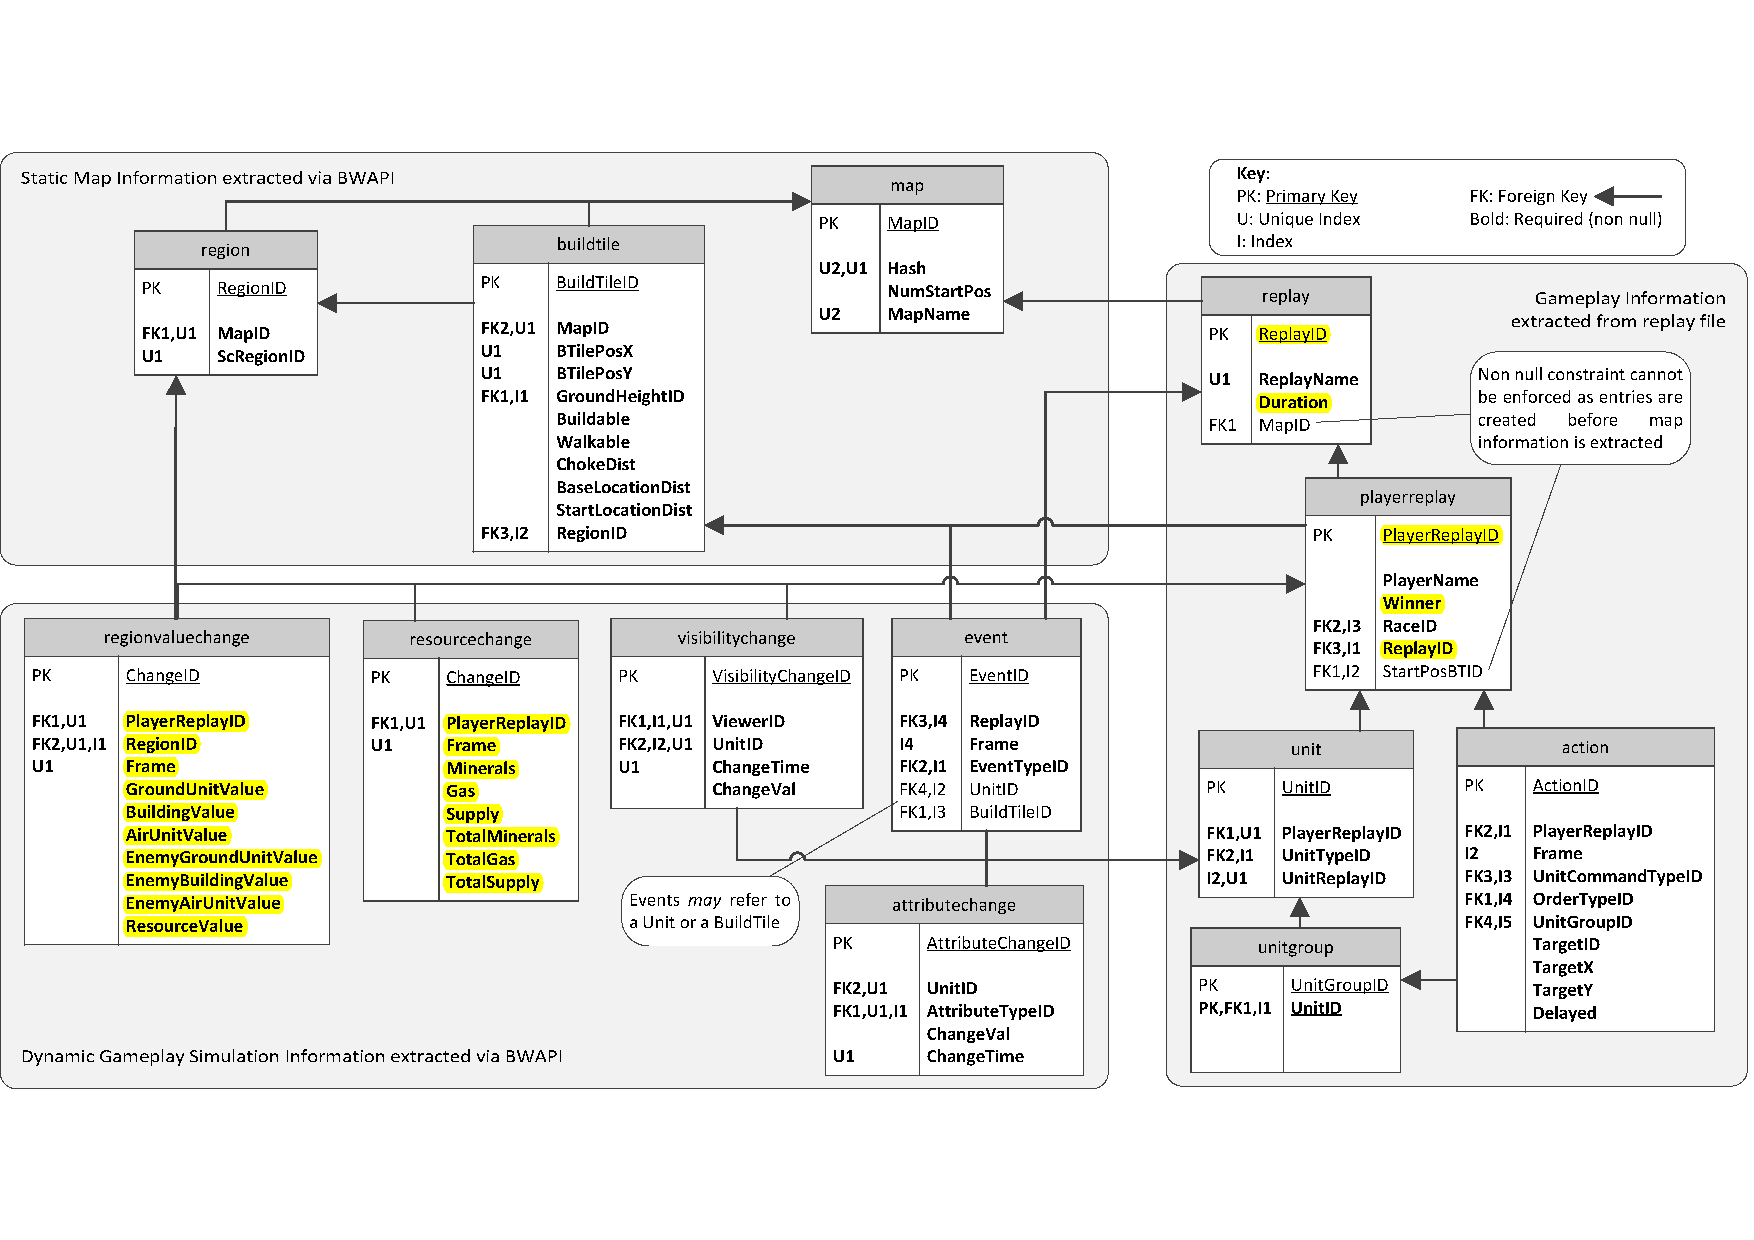
\includegraphics[scale=0.5]{figure/Robertson14DatabaseDiagramSeleccion.pdf}
  \caption{Selected features in databases. Original diagram by~\cite{DBLP:conf/flairs/RobertsonW14}}
  \label{fig:databaseSelection}
\end{figure*}

We present here the list of selected features, also exposed in
Figure~\ref{fig:databaseSelection}. Some of them are used only to organise the
data, the identifiers of replay, player and region.

\begin{itemize}
  \item replay: Contains data about each match.
  \begin{itemize}
    \item ReplayID: Match identifier.
    %\item Duration: Duration of each match in frames, 15 frames per second.
  \end{itemize}
  \item playerreplay: Contains data about a player in a match.
  \begin{itemize}
    \item PlayerReplayID: Player identifier.
    \item ReplayID: Match identifier.
    \item Winner: Winner of the match.
  \end{itemize}
  \item resourcechange: Contains data associated to changes in player's resources.
  \begin{itemize}
    \item PlayerReplayID: Player identifier.
    \item Frame: Frame when the resource changes.
    \item Minerals: Amount of minerals of a player.
    \item Gas: Amount of gas of a player.
    \item Supply: Carrying capacity of a player.
    \item TotalMinerals: Total amount of minerals of a player, without costs.
    \item TotalGas: Total amount of gas of a player, without costs.
    \item TotalSupply: Total amount of supply of a player, without costs.
  \end{itemize}
  \item regionvaluechange: Contains data associated to changes of a
  player in a map region. Each \emph{value} is the sum of the price of an unit,
  expressed as minerals and gas.
  \begin{itemize}
    \item PlayerReplayID: Player identifier.
    \item RegionID: Region of the map identifier.
    \item Frame: Frame when the value changes.
    \item GroundUnitValue: Value of ground units in this region.
    \item BuildingValue: Value of buildings in this region.
    \item AirUnitValue: Value of air units in this region.
    \item EnemyGroundUnitValue: Value of enemy ground units in this region.
    This value is estimated, the player knows the units they see of the enemy.
    \item EnemyBuildingValue: Value of enemy buildings in this region.
    This value is estimated, the player knows the units they see of the enemy.
    \item EnemyAirUnitValue: Value of enemy air units in this region.
    This value is estimated, the player knows the units they see of the enemy.
    \item ResourceValue: Value of resources in this region. This value is
    estimated, the player knows the units they see of the map.
    If the player does not know a region, they estimate this value as the maximum
    available in the region.
  \end{itemize}
\end{itemize}

The features related to a player are presented twice, one for each player.
Furthermore, a \emph{race} feature is used, as the races implied in the match.
As a consequence, we have 28 features used in the modelling stage of the work.

\subsection{Data preprocessing}
\label{subsec:preprocess}

As we said in Section~\ref{subsec:selection}, each observation of the data has 28
features related to the resources and units of each player. We have to note
some little tips about the data organisation.

\begin{itemize}
  \item Values of \emph{Frame} are the instants when any player has
  a minerals, gas or supply change. We did this election because in these games
  the basic resources are always changing due to necessity of them to buy
  units or buildings. This implies some missing values in the resources of
  the player who doesn't make a change in that frame, so we had to recover the
  last value of that resource to keep consistency.
  \item Values of \emph{value} of units and buildings changes do not occur in the
  same instant that the resources' changes. For this reason, as we did with
  \emph{Frame}, we had to recover the last \emph{value} of the region
  \emph{values} of each player, too.
  \item \emph{Value} depends of the region of the map. It's important in our
  approach to get a full \emph{value} measure, a value that represents all
  the player units or buildings, so we had to sum the \emph{value} of every
  region of the map.
\end{itemize}


% \subsection{Exploratory Data Analysis}
% \label{subsec:eda}

\subsection{Modelling}
\label{subsec:modelling}

We have chosen six algorithms for the modelling. Some of them are very simple,
because we want to test if a simple algorithm can model the data.

\begin{itemize}
  \item \emph{Naive Bayes} (NB)
  \item \emph{Logistic Regression} (LR)
  \item \emph{KNN} (KNN)
  \item \emph{Multilayer perceptron} (MLP)
  \item \emph{Random Forest} (RF)
  \item \emph{Gradient Boosting Tree} (GBT)
\end{itemize}

The final results are obtained using this approach 5 times:

\begin{enumerate}
  \item Split data using 70\% to train and 30\% to validation.
  \item Inside the first partition, train a model using 10-fold Cross Validation.
  \item With the final model, validate it in the second partition.
\end{enumerate}

Using this approach, we get 5 accuracy measures for each model, so we can test
the obtained samples using appropiate statistical tests. We use \emph{Friedman
test} to get statistical differences among all the classifiers, and a
pairwise \emph{t-test} to get differences between classifiers.

\section{\uppercase{Results}}
\label{sec:results}

In Figure~\ref{fig:MeasuresGraphics} and Table~\ref{tab:measures} is
exposed the accuracy of each model with their parameters. The accuracy is
evaluated in the validation sets.



Median with standard deviation is shown because data is not centered around the
mean in all the selected instants.

% latex table generated in R 3.2.3 by xtable 1.8-2 package
% Mon Sep  4 23:23:53 2017
\begin{table*}[ht]
\centering
\begin{tabular}{rlrrl}
  \hline
 & Classifier & Accuracy & SD & Params \\ 
  \hline
1 & GBT & 0.859000 & 0.002563 & numTrees = 150, maxDepth = 10 \\ 
  2 & KNN & 0.975589 & 0.000091 & K = 3 \\ 
  3 & LR & 0.613878 & 0.000294 & maxIter = 150, regParam = 0.3 \\ 
  4 & MLP & 0.626332 & 0.010706 & Hidden layers = (10,10) \\ 
  5 & NB & 0.507295 & 0.000550 & Smoothing = 1 \\ 
  6 & RF & 0.680166 & 0.000474 & numTrees = 150, maxDepth = 10 \\ 
   \hline
\end{tabular}
\caption{Trained algorithms with their final parameters} 
\label{tab:measures}
\end{table*}


In general, all classifiers but \emph{Naive Bayes} predict pretty well, but
there are two clear winners: \emph{Gradient Boosting Tree} and \emph{KNN}.
This one offers a great accuracy with a very simple approach, but it is not
suitable for doing a lot of predictions in real time, because of its lazy
approach.

%\begin{knitrout}
\definecolor{shadecolor}{rgb}{0.969, 0.969, 0.969}\color{fgcolor}
\begin{figure*}[h!tb]
\includegraphics[width=\maxwidth]{figure/MeasuresGraphics-1} \caption[Measures obtained with all models]{Measures obtained with all models}\label{fig:MeasuresGraphics}
\end{figure*}


%\end{knitrout}

%\begin{knitrout}
\definecolor{shadecolor}{rgb}{0.969, 0.969, 0.969}\color{fgcolor}
\begin{figure*}[h!tb]
\includegraphics[width=\maxwidth]{figure/TimeComparisonAcc-1} \caption[Comparing classifiers over time]{Comparing classifiers over time}\label{fig:TimeComparisonAcc}
\end{figure*}


%\end{knitrout}

In Figure~\ref{fig:TimeComparisonAcc} is exposed the accuracy differences
between classifiers over time. \emph{KNN} can classify with a precision of $0.902 \pm \ensuremath{3.292\times 10^{-4}}$ only
with 10 minutes of match. The mean of the duration is \ensuremath{4.397\times 10^{4}}
frames, which are equal to 48.854 minutes. It implies that
with only a 20.469\% of the mean duration
of the match, we can predict accurately the winner of a match. It is not
necessary to play the whole match to get the winner with high confidence.

To complete the study, we present a Friedman test to see significative
differences over the classifiers. All frames of the matches are used. We
can see in Table~\ref{tab:acc} the accuracy of each classifier.

% latex table generated in R 3.2.3 by xtable 1.8-2 package
% Mon Sep  4 23:23:54 2017
\begin{table*}[ht]
\centering
\begin{tabular}{rrrrrrr}
  \hline
 & RF & LR & NB & GBT & MLP & KNN \\ 
  \hline
1 & 0.680004 & 0.613650 & 0.507551 & 0.859000 & 0.605377 & 0.975575 \\ 
  2 & 0.680166 & 0.614189 & 0.508414 & 0.854445 & 0.626332 & 0.975589 \\ 
  3 & 0.679876 & 0.613430 & 0.507042 & 0.860723 & 0.628845 & 0.975416 \\ 
  4 & 0.681080 & 0.613981 & 0.507155 & 0.856990 & 0.611386 & 0.975620 \\ 
  5 & 0.680194 & 0.613878 & 0.507295 & 0.860127 & 0.627228 & 0.975652 \\ 
   \hline
\end{tabular}
\caption{Accuracy of classifiers in each validation set} 
\label{tab:acc}
\end{table*}


With a p-value of \ensuremath{1.889\times 10^{-4}}, we can confirm that statistical
signification exists. We can see in Table~\ref{tab:pvalues} a pairwise test, with
\emph{Bonferroni} adjust method of the p-value.

% latex table generated in R 3.2.3 by xtable 1.8-2 package
% Mon Sep  4 23:23:54 2017
\begin{table*}[ht]
\centering
\begin{tabular}{rrrrrr}
  \hline
 & RF & LR & NB & GBT & MLP \\ 
  \hline
LR & 0.000000 &  &  &  &  \\ 
  NB & 0.000000 & 0.000000 &  &  &  \\ 
  GBT & 0.000000 & 0.000000 & 0.000000 &  &  \\ 
  MLP & 0.000486 & 0.277633 & 0.000058 & 0.000004 &  \\ 
  KNN & 0.000000 & 0.000000 & 0.000000 & 0.000000 & 0.000001 \\ 
   \hline
\end{tabular}
\caption{p-values from a pairwise t-test} 
\label{tab:pvalues}
\end{table*}


As we can see, we can confirm that with the usual signification level, 0.05,
there are statistical differences among all classifiers but \emph{Logistic
Regression} and \emph{Multilayer Perceptron}. They are not the best classifiers
so this is not important. The important fact is that there are statistical
differences between \emph{KNN} and \emph{Gradient Boosting Tree}.

\section{\uppercase{Conclusions}}
\label{sec:conclusions}

With this study we can extract some conclusions. The first one is that the set
of features is well formed: the winner can be predicted from the selected
features with high confidence, as we exposed in Section~\ref{sec:results}.

The second and main conclusion is that predictions with this data are very
accurate in an early stage, in particular using a \emph{KNN}
classifier. It can predict with 90\% of accuracy using 10 minutes of match only. % How much as a percentage of the total time? 
This is very important because it proves that it is not necessary to play a
whole match to predict the winner accurately. % How much does it need to play?

% This means that current simulations which take... will need only ... 

This predicted performance of bots can be used for surrogate models \cite{zhou2007combining} that will allow faster evaluation; these fast evaluations can be combined with real ones if needed. 

As future work there are some research opportunities using this study. With a
\emph{KNN} classifier, a competitive \emph{bot} could be developed with an
important skill: the winner's prediction. It could be used to improve the
adaptability of the agent, giving advantage to its opponents.

Another work could be the improvement of \emph{bot} optimization using the early
winner knowledge. We could use this knowledge to improve the evaluation step of
the algorithms, giving the opportunity to use more exhaustive setups on the
algorithms.





\section*{\uppercase{Acknowledgements}}
\label{sec:acknowledgements}

This work has been supported in part by: de Ministerio espa\~{n}ol de
Econom\'{\i}a y Competitividad under project TIN2014-56494-C4-3-P
(UGR-EPHEMECH) and by CONACYT PEI Project No. 220590.

\vfill
\bibliographystyle{apalike}
{\small
\bibliography{prediction}}

\vfill
\end{document}
